
\begin{table}[H]
\centering
\begin{tabular}{lllllll}
\textbf{Rows} & \textbf{1} & \textbf{10} & \textbf{100} & \textbf{1000} & \textbf{10000} & \textbf{100000} \\
\textbf{Initial pull} & 391.97 & 378.33 & 224.64 & 51.19 & 5.81 & 0.54\\
\textbf{Pull 1 change} & 455.58 & 449.93 & 386.48 & 173.35 & 19.53 & 0.96\\
\textbf{Pull 10 changes} & 415.95 & 395.61 & 360.66 & 167.17 & 19.41 & 0.95\\
\textbf{Pull 100 changes} & 240.27 & 236.6 & 218.29 & 127.87 & 18.22 & 0.95\\
\textbf{Create reservation} & 363.92 & 365.95 & 361.59 & 369.67 & 318.99 & 120.61\\
\textbf{Update reservation} & 716.35 & 728.02 & 718.99 & 717.93 & 722.39 & 703.58\\
\textbf{Delete reservation} & 759.92 & 763.04 & 756.66 & 759.39 & 762.33 & 736.68
\end{tabular}
\caption{Througput in requests per second for server-side operations per number of rows in client state.}
\label{tab:server-relic-experiment}
\end{table}

\begin{table}[H]
\centering
\begin{adjustbox}{width=\textwidth}
\begin{tabular}{lllllll}
\textbf{Rows} & \textbf{1} & \textbf{10} & \textbf{100} & \textbf{1000} & \textbf{10000} & \textbf{100000} \\
\textbf{Initial pull} & 254.39 (292.4) & 263.51 (287.7) & 443.28 (475.27) & 1924.03 (2036.19) & 15403.87 (21603.3) & 131028.92 (200721.72)\\
\textbf{Pull 1 change} & 217.02 (241.76) & 219.57 (236.99) & 254.68 (280.3) & 550.57 (599.86) & 3745.7 (4268.9) & 23092.33 (44488.38)\\
\textbf{Pull 10 changes} & 237.57 (258.45) & 249.65 (275.31) & 273.13 (298.07) & 570.79 (616.28) & 3782.62 (4355.26) & 23183.93 (45231.95)\\
\textbf{Pull 100 changes} & 410.59 (443.82) & 416.52 (448.84) & 449.91 (486.53) & 744.6 (812.69) & 3987.88 (4601.86) & 23253.35 (45270.12)\\
\textbf{Create reservation} & 270.72 (344.7) & 269.44 (349.2) & 272.64 (360.44) & 266.65 (354.79) & 308.69 (387.15) & 805.18 (879.77)\\
\textbf{Update reservation} & 138.14 (147.76) & 135.87 (144.5) & 137.57 (147.16) & 137.79 (147.38) & 136.8 (145.06) & 138.95 (147.55)\\
\textbf{Delete reservation} & 130.18 (138.94) & 129.65 (137.13) & 130.7 (138.93) & 130.27 (138.4) & 129.62 (137.82) & 132.7 (141.42)
\end{tabular}
\end{adjustbox}
\caption{Average latency in milliseconds for server-side operations per number of rows in client state. The 95th percentile of latency is shown in parentheses.}
\label{tab:server-relic-experiment-latency}
\end{table}

\begin{figure}[H]
    \centering

\begin{subfigure}[b]{0.48\textwidth}
    \centering
    
\resizebox{\textwidth}{!}{
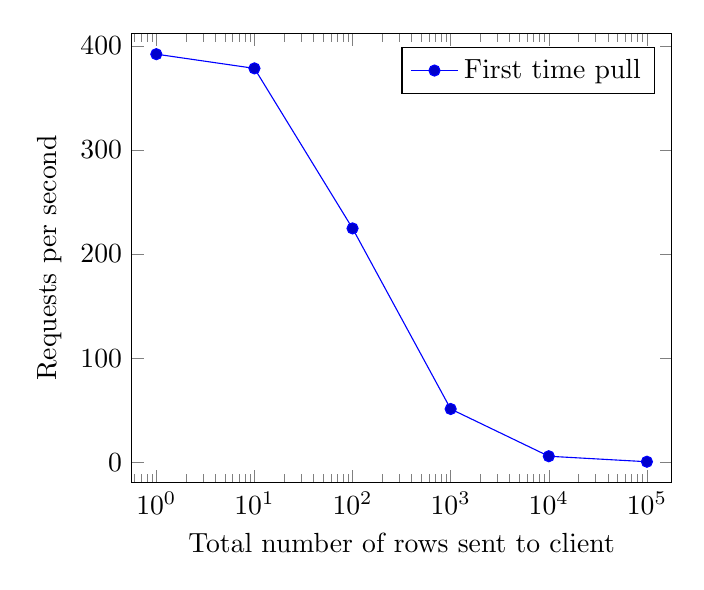
\begin{tikzpicture}
\begin{axis}[
    scaled x ticks=false,
    xticklabel style={
        /pgf/number format/fixed,
    },
    enlargelimits=0.05,
    xmode=log,
    legend pos=north east,
	ylabel=Requests per second,
    xlabel=Total number of rows sent to client,
]
\addplot coordinates {
(1,391.96970573279566)
(10,378.3253756250079)
(100,224.64484496588693)
(1000,51.19365057514714)
(10000,5.813816724676129)
(100000,0.5369540107640169)
};
\legend{First time pull}
\end{axis}
\end{tikzpicture}

}

    \caption{Throughput in requests per second for the first pull of a new client.}
    \label{fig:server-initial-pull}
\end{subfigure}
\hfill
\begin{subfigure}[b]{0.48\textwidth}
    \centering
    
\resizebox{\textwidth}{!}{
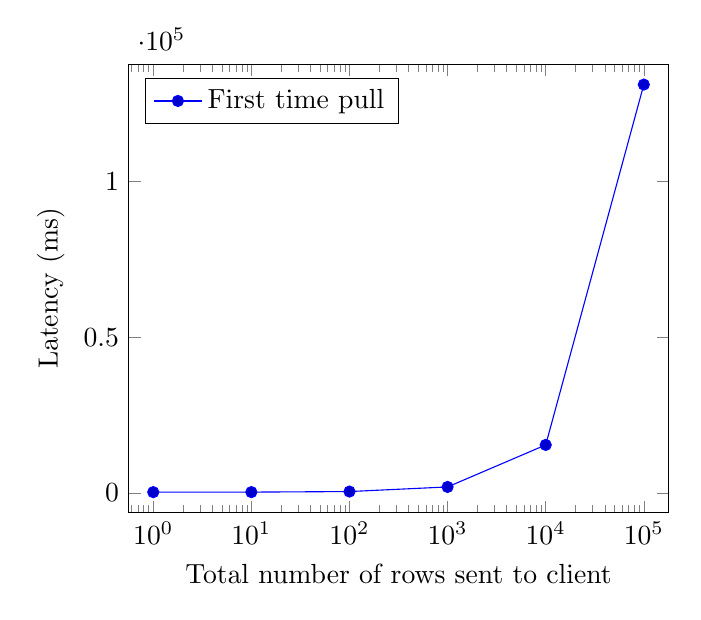
\begin{tikzpicture}
\begin{axis}[
    scaled x ticks=false,
    xticklabel style={
        /pgf/number format/fixed,
    },
    enlargelimits=0.05,
    xmode=log,
    legend pos=north west,
	ylabel=Latency (ms),
    xlabel=Total number of rows sent to client,
]
\addplot coordinates {
(1,254.38983778511715)
(10,263.50984867731563)
(100,443.28321901444366)
(1000,1924.0289357299423)
(10000,15403.867151386516)
(100000,131028.92420834785)
};
\legend{First time pull}
\end{axis}
\end{tikzpicture}

}

    \caption{Latency in milliseconds for the first pull of a new client.}
    \label{fig:server-initial-pull-latency}
\end{subfigure}
\\
\begin{subfigure}[b]{0.48\textwidth}
    \centering
    
\resizebox{\textwidth}{!}{
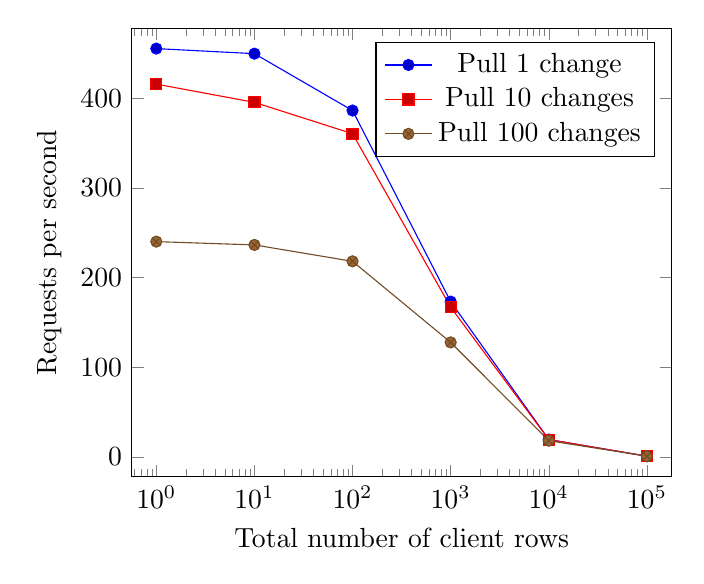
\begin{tikzpicture}
\begin{axis}[
    scaled x ticks=false,
    xticklabel style={
        /pgf/number format/fixed,
    },
    enlargelimits=0.05,
    xmode=log,
    legend pos=north east,
	ylabel=Requests per second,
    xlabel=Total number of client rows,
]
\addplot coordinates {
(1,455.57718447966516)
(10,449.9276399515963)
(100,386.476556794098)
(1000,173.34755875653505)
(10000,19.52731147591755)
(100000,0.9566121823784789)
};
\addplot coordinates {
(1,415.9467521803226)
(10,395.60791394673595)
(100,360.65523962398646)
(1000,167.17490884186375)
(10000,19.410548784976424)
(100000,0.9530903479837194)
};
\addplot coordinates {
(1,240.26929636687962)
(10,236.59645085179926)
(100,218.28651428010465)
(1000,127.87032160125923)
(10000,18.224891026773232)
(100000,0.9465681752846462)
};
\legend{Pull 1 change,Pull 10 changes,Pull 100 changes}
\end{axis}
\end{tikzpicture}

}

    \caption{Throughput for subsequent pulls of clients for N changed rows.}
    \label{fig:server-pull-n}
\end{subfigure}
\hfill
\begin{subfigure}[b]{0.48\textwidth}
    \centering
    
\resizebox{\textwidth}{!}{
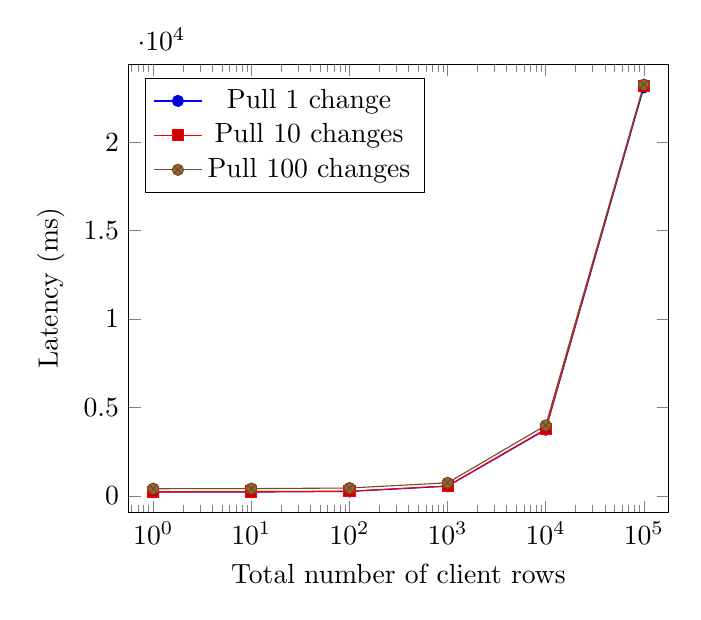
\begin{tikzpicture}
\begin{axis}[
    scaled x ticks=false,
    xticklabel style={
        /pgf/number format/fixed,
    },
    enlargelimits=0.05,
    xmode=log,
    legend pos=north west,
	ylabel=Latency (ms),
    xlabel=Total number of client rows,
]
\addplot coordinates {
(1,217.01545544799154)
(10,219.57330747412)
(100,254.68337207021995)
(1000,550.5720499571339)
(10000,3745.70231154583)
(100000,23092.325037811268)
};
\addplot coordinates {
(1,237.56725457737508)
(10,249.65486637276587)
(100,273.1270779137456)
(1000,570.7942191220385)
(10000,3782.6222167889337)
(100000,23183.927247033345)
};
\addplot coordinates {
(1,410.5926733855004)
(10,416.52272880117823)
(100,449.9107454482832)
(1000,744.5978975732444)
(10000,3987.880486395787)
(100000,23253.35030110962)
};
\legend{Pull 1 change,Pull 10 changes,Pull 100 changes}
\end{axis}
\end{tikzpicture}

}

    \caption{Latency in milliseconds for subsequent pulls of clients for N changed rows.}
    \label{fig:server-pull-n-latency}
\end{subfigure}
\\
\begin{subfigure}[b]{0.48\textwidth}
    \centering
    
\resizebox{\textwidth}{!}{
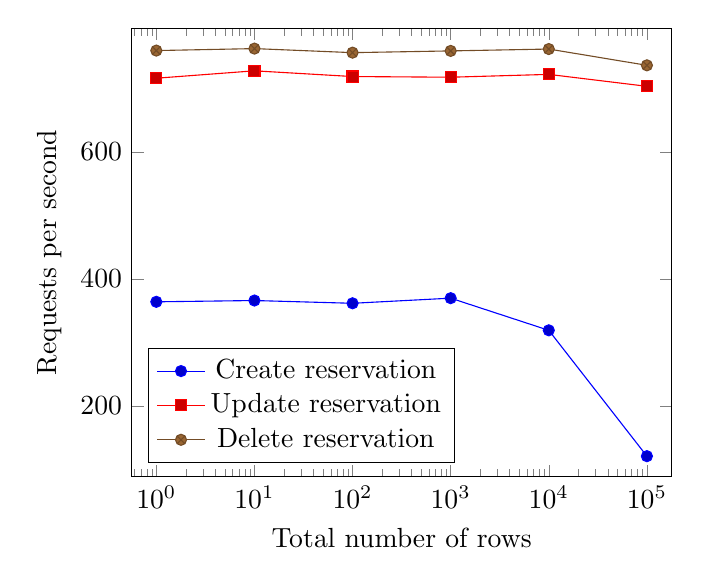
\begin{tikzpicture}
\begin{axis}[
    scaled x ticks=false,
    xticklabel style={
        /pgf/number format/fixed,
    },
    enlargelimits=0.05,
    xmode=log,
    legend pos=south west,
	ylabel=Requests per second,
    xlabel=Total number of rows,
]
\addplot coordinates {
(1,363.9183465561893)
(10,365.9513168286966)
(100,361.592664717432)
(1000,369.6694166949371)
(10000,318.98789721440147)
(100000,120.60599135923887)
};
\addplot coordinates {
(1,716.3481557213865)
(10,728.0194418331411)
(100,718.9949732945853)
(1000,717.9307876660754)
(10000,722.3897497394355)
(100000,703.5825817842272)
};
\addplot coordinates {
(1,759.9216077231771)
(10,763.0356848893141)
(100,756.6568914293897)
(1000,759.3936183353776)
(10000,762.3278571020595)
(100000,736.6820704731044)
};
\legend{Create reservation,Update reservation,Delete reservation}
\end{axis}
\end{tikzpicture}

}

    \caption{Throughput for pushing mutations to the server.}
    \label{fig:server-push}
\end{subfigure}
\hfill
\begin{subfigure}[b]{0.48\textwidth}
    \centering
    
\resizebox{\textwidth}{!}{
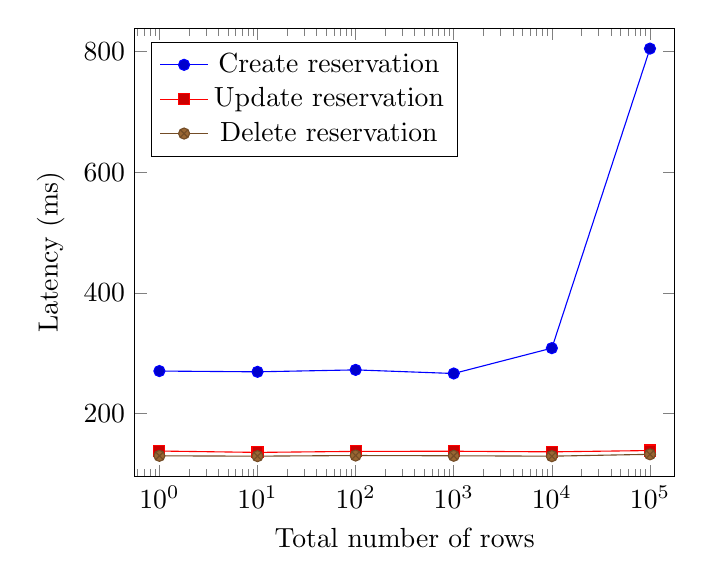
\begin{tikzpicture}
\begin{axis}[
    scaled x ticks=false,
    xticklabel style={
        /pgf/number format/fixed,
    },
    enlargelimits=0.05,
    xmode=log,
    legend pos=north west,
	ylabel=Latency (ms),
    xlabel=Total number of rows,
]
\addplot coordinates {
(1,270.7156683916384)
(10,269.4359520401143)
(100,272.6356202451486)
(1000,266.6530386619228)
(10000,308.6938787735821)
(100000,805.1835728009075)
};
\addplot coordinates {
(1,138.13863232297297)
(10,135.86679343577345)
(100,137.56826389910532)
(1000,137.79169962761384)
(10000,136.80263658800783)
(100000,138.95000097028625)
};
\addplot coordinates {
(1,130.1778916211859)
(10,129.64517954295496)
(100,130.6992538247182)
(1000,130.2725272440822)
(10000,129.61781922784024)
(100000,132.70423946248695)
};
\legend{Create reservation,Update reservation,Delete reservation}
\end{axis}
\end{tikzpicture}

}

    \caption{Latency in milliseconds for pushing mutations to the server.}
    \label{fig:server-push-latency}
\end{subfigure}
    
    \caption{Throughput of server for handling pull and push requests by total number of rows in client state.}
    \label{fig:server-relic-experiment}
\end{figure}
